\chapter{Approach} \label{c:approach}

In this section after describing the general convolutional architecture in spiking neural network, to find the best performing spiking convolutional DBN, we discuss two different approaches to build these.

The first one is the more classical one, where a in discrete time trained DBN is transferred to spiking neural networks.
The second approach trains the RBMs event based with STDP directly as spiking neural networks. 

In Chapter \ref{c:expres}, we will then evaluate and compare the performance of both approaches.

\section{Convolutional architecture in spiking neural network} \label{c:spikingconvarch}

We implement a convolutional layer with receptive fields and shared weights between two neuron populations. 
Each population has a similar three dimensional topology as in "normal" CNNs with the number of neurons given by $n_{ \text{neurons}} = \text{channels} \times \text{height} \times \text{width}$.

Groups of neurons in the bottom layer in close vicinity, a so-called receptive fields, are each connected with synapses to the same top layer neuron (see Fig. \ref{fig:receptfields1}).
These receptive fields have the same shape and size $n$ and share the same synaptic weights (given the top layer neurons belong to the same feature map).
Adjacent receptive fields are overlapping by one neuron and the output neurons have the same topology as their input regions. 

A receptive field covers a partial region of the input data and the synaptic weights from the bottom layer neurons to the top layer neuron can the be seen as a convolution over the partial input data.
Since the weights of the receptive field can be shared, the neural activity in the top layer can be seen as a convolution over the input data with a filter of the size of the receptive fields.
In this case the top layer activation of receptive fields with the same weights can also be called a feature map  (see Fig. \ref{fig:receptfields2}).
By using more neurons with different set of shared weights over the same receptive fields, more feature maps can be implemented.     

\begin{figure}
	\centering
	\begin{subfigure}[t]{.5\textwidth}
  		\centering
  		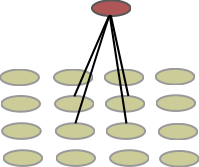
\includegraphics[width=.8\linewidth]{imgs/recpt_field1.png}
  		\caption{A singe receptive field over 4 neurons}
  		\label{fig:receptfields1}
	\end{subfigure}%
	\begin{subfigure}[t]{.5\textwidth}
  		\centering
  		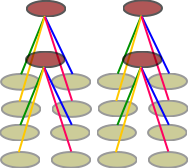
\includegraphics[width=.8\linewidth]{imgs/recpt_field2.png}
  		\caption{Four receptive fields with shared weights.}
  		\label{fig:receptfields2}
	\end{subfigure}
	\caption{Receptive fields over 4 neurons. In (a) the top layer neuron (red), is only connected to a some neurons in close vicinity to each other. In (b) four receptive fields are next to each other with a stride of two and shared weights. The top layer neurons have a similar topology as their receptive fields. Such a structure can give similar results to conventional more dimensional convolution. }
	\label{fig:receptfields}
\end{figure}




\section{Conversion} \label{c:convappro}

The conversion approach can be roughly described in two steps:
\begin{enumerate}
\item Train the RBMs to build up an DBN.
\item Convert the DBN to the spiking neural network.
\end{enumerate}


\subsection{Convolutional DBNs} \label{c:convdbns}

To train a convolutional DBNs we proceed similar to Hinton et al. and Lee et al. \cite{hinton2006fast} \cite{lee2009convolutional}.

At first the convolutional RBMs are trained greedily with CD, as described in Chapter \ref{c:convrbm}, for a certain number of iterations on data batches of batch-size $b$.
After a RBM is trained, we convert the dataset by sampling of the hidden layer of the RBM (one sampling/forward-pass step), into a new dataset:
\[
p(x') = \sigma(W * x) .
\]

On this converted dataset the next convolutional RBM is trained similar to the previous one.

Evaluating feature qualities is still an active research topic.
To get a measurement of our feature quality we use labelled data and train a classifier on top of the extracted features.
To stay in a biological plausible domain, we train a fully connected RBM on the top level features as well as the label of the data samples, to associate the features with the correct labels.
This architecture is similar to the architecture of Hinton \cite{hinton2006fast} (see Fig. \ref{fig:dbnmnist}).

\begin{figure}
	\centering
    	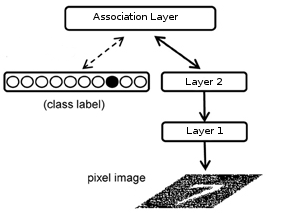
\includegraphics[width=0.4\textwidth]{imgs/dbn_mnist.png} 
    \caption{A common structure of a deep belief network, built up of RBMs used for classification. The first layers transform the input data/ pixel image and can extract features and the top layer RBM is used for association the data with the correct label.}
	\label{fig:dbnmnist}
\end{figure}

To evaluate the final performance, we input a data sample without a label into the DBN and let the top layer sample a label prediction by performing Gibbs sampling steps, which can be seen as a reconstruction of partially presented data (as mentioned in Chapter \ref{c:pgms}).


\subsection{Conversion} \label{c:conversionappr}

For the conversion we present three different variations.

\begin{figure}
	\centering
	\begin{subfigure}[t]{.5\textwidth}
  		\centering
  		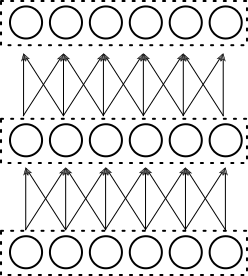
\includegraphics[width=.6\linewidth]{imgs/convert_cnn.png}
  		\caption{Structure of a spiking CNN with LIF neurons.}
  		\label{fig:converted1}
	\end{subfigure}%
	\begin{subfigure}[t]{.5\textwidth}
  		\centering
  		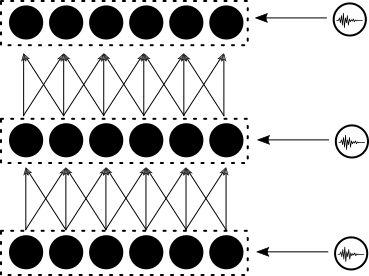
\includegraphics[width=.8\linewidth]{imgs/convert_dbn.png}
  		\caption{Structure of a spiking DBN with LIF neurons.}
  		\label{fig:converted2}
  	\end{subfigure}
	\caption{Different converted structures of a CNN and a DBN. The CNN is converted to a spiking network, by simply using simple LIF neurons (white) (a). In the DBN (b) the LIF neurons are put in a high conductance state (black), by inserting high frequency Poisson noise. The weights are scaled accordingly to fit the activations of the neurons.}
	\label{fig:converted}
\end{figure}


\paragraph{Conversion as CNN}  \label{c:convascnn}

One way to convert the DBN to the spiking domain, is by interpreting it as a pre-trained CNN with purely forward connections (we do not perform any commonly used gradient descent fine tuning to get comparable results with only CD trained models, but fine tuning could further improve the performance).
While this allows classification, it removes the generative capabilities of the network.

For the conversion, we proceed similar to Cao et al. and Diehl et al. \cite{Cao2014} \cite{Diehl2015} .
They use average pooling and ReLU functions, to get a similar architecture as SNNs.
In contrast, we don't use any pooling, since for RBM there is no simple way to integrate average pooling (used by Cao and Diehl in their trained CNNs), and for spiking CNNs there is no simple way to integrate probabilistic max pooling, which is to our knowledge currently the only training integrated pooling thought of for RBMs.
We also use the sigmoid function, since RBMs are commonly trained with sigmoid activations (but some approaches propose ReLU for RBMs as well \cite{Nair2010}).
Furthermore the input-rate output-rate transfer function of rate based LIF neurons with a refractory period matches the sigmoid function more closely.

The DBN layers are replaced by a LIF neuron population layers with an identical architecture (see Fig. \ref{fig:converted1}). 
The connections are replaced by (directed) synapses, with the weights of the DBN synapses scaled with a constant factor, to get similar activations.
 

\paragraph{Conversion with conductance-based LIF} \label{c:convascoba}

Another way to convert the DBN to the spiking domain, is by interpreting it as a directed graphical model, a sigmoid belief network, and performing ancestral sampling.
This approach is heavily based on the synaptic sampling theory, i.e. it uses spiking neurons to perform sampling.
The sampling can be either performed with current-based or conductance-base LIF neurons as described in Chapter \ref{c:snnsampling}.

For the COBA neurons, we choose a biological plausible neuron model (see parameters in Table \ref{cobalifparam}). 
The high membrane conductance, an increased Gaussian distributed mean membrane potential and thus a firing probability of $0.5$, is achieved by using high frequency Poisson generated inhibitory and excitatory spikes to bring the neuron to a high conductance state (HCS) (see Fig. \ref{fig:cobahcs1}). 
This neuron model has an input-rate output-rate transfer function which approximates a sigmoid function (see Fig. \ref{fig:cobahcs2}).

The PSPs are chosen to have an alpha shape instead of rectangular shape, which as described in Chapter \ref{c:snnsampling} may introduce some discrepancies when performing sampling in comparison to Gibbs sampling, but is more biologically plausible (see Fig. \ref{fig:cobahcs3}).

\begin{figure}
	\centering
	\begin{subfigure}[t]{.5\textwidth}
  		\centering
  		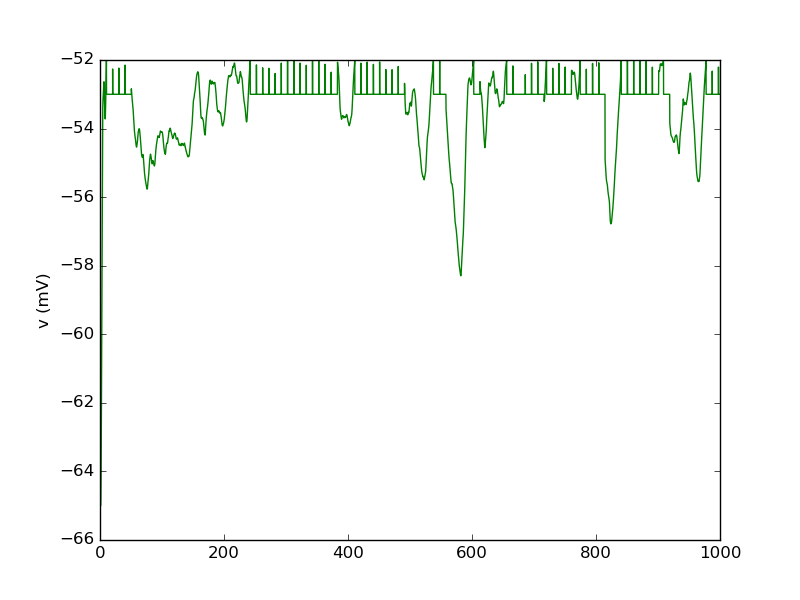
\includegraphics[width=.8\linewidth]{imgs/coba_lif_act.png}
  		\caption{Firing of a HCS COBA LIF neuron.}
  		\label{fig:cobahcs1}
	\end{subfigure}%
	\begin{subfigure}[t]{.5\textwidth}
  		\centering
  		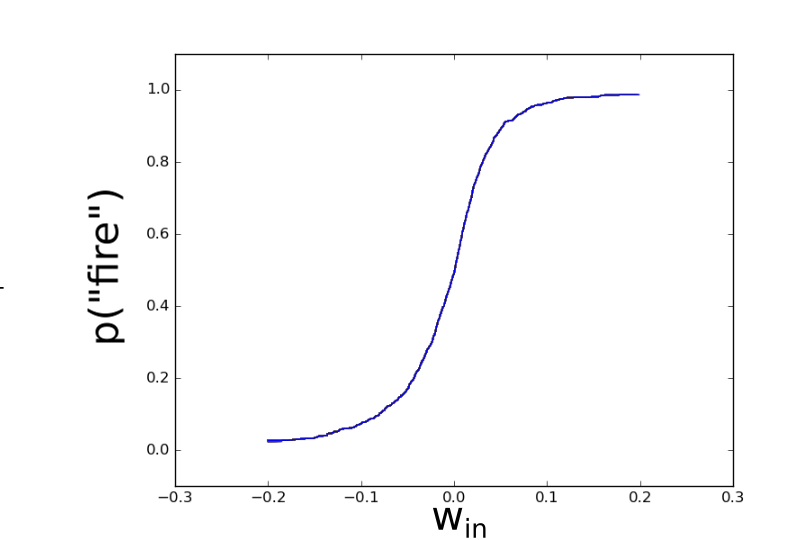
\includegraphics[width=.8\linewidth]{imgs/coba_lif_sigmoid.png}
  		\caption{Input output transfer function of a HCS COBA LIF neuron.}
  		\label{fig:cobahcs2}
	\end{subfigure}
	\begin{subfigure}[t]{.5\textwidth}
  		\centering
  		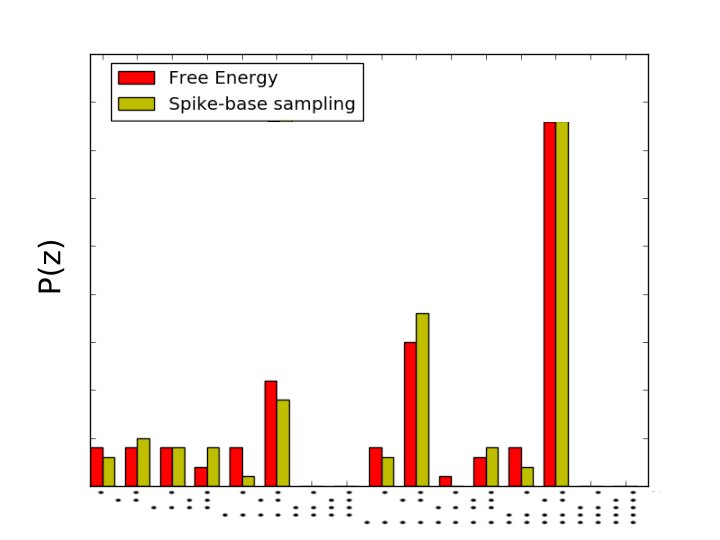
\includegraphics[width=.8\linewidth]{imgs/coba_lif_bm2.png}
  		\caption{omparison between a HCS COBA LIF neuron sampling and the true distribution in a RBM.}
  		\label{fig:cobahcs3}
	\end{subfigure}
	\caption{Properties of a conductance based LIF neuron, put into a high conductance state with high frequency input noise. The neuron fires with a probability of $0.5$ given no additional input (a). With input the input output transfer function approximates a sigmoid function (b). A network with such neurons is able to sample in a Boltzmann distribution similar to original distribution (c). }
	\label{fig:cobahcs}

\end{figure}
  
The DBN is converted by simply converting each layer to a layer of conductance-based LIF neurons with Poisson noise, and the connections are transformed to synapses with the weights scaled to achieve a action function similar to the sigmoid function (see Fig. \ref{fig:converted2}).

Consequently the DBN simply performs ancestral sampling with the data sample as evidences and the label as inferred state.   


\paragraph{Conversion with current-based LIF} \label{c:convascuba}

To reduce the computational expenses of the COBA models, they can be replaced by less computational complex CUBA models.
The model parameters as chose to simulate a HCS state.
Therefore the membrane time constant is reduced as well as the membrane conductance increased and a static input current is inserted.  
By adding high frequency Poisson noise, a sigmoid shaped input-rate output-rate transfer function is achieved (see Fig. \ref{fig:cubahcs}).

\begin{figure}
	\centering
	\begin{subfigure}[t]{.5\textwidth}
  		\centering
  		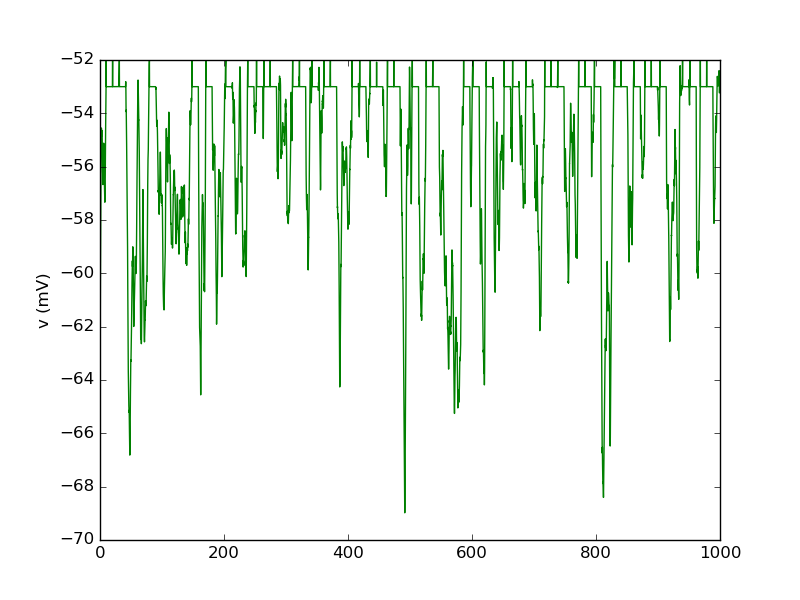
\includegraphics[width=.8\linewidth]{imgs/cuba_lif_act.png}
  		\caption{Firing of a HCS CUBA LIF neuron.}
  		\label{fig:sub1}
	\end{subfigure}%
	\begin{subfigure}[t]{.5\textwidth}
  		\centering
  		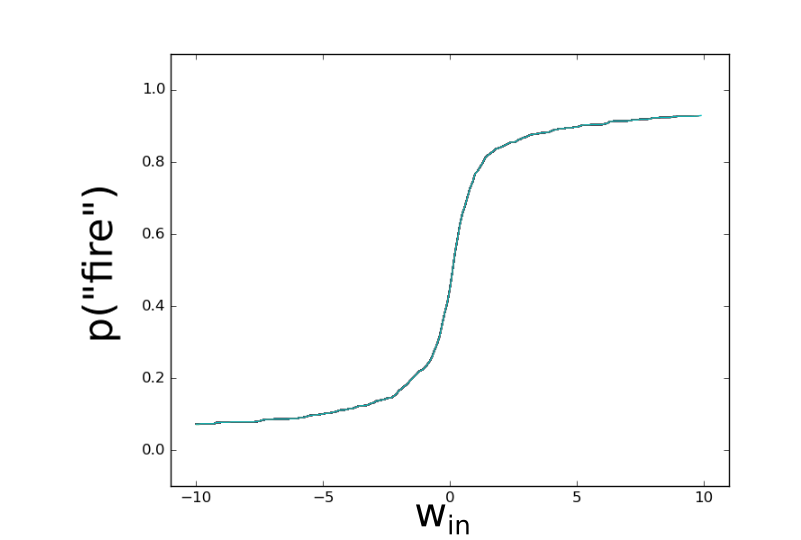
\includegraphics[width=.8\linewidth]{imgs/cuba_lif_sigmoid.png}
  		\caption{Input output transfer function of a HCS CUBA LIF neuron.}
  		\label{fig:sub2}
	\end{subfigure}
	\begin{subfigure}[t]{.5\textwidth}
  		\centering
  		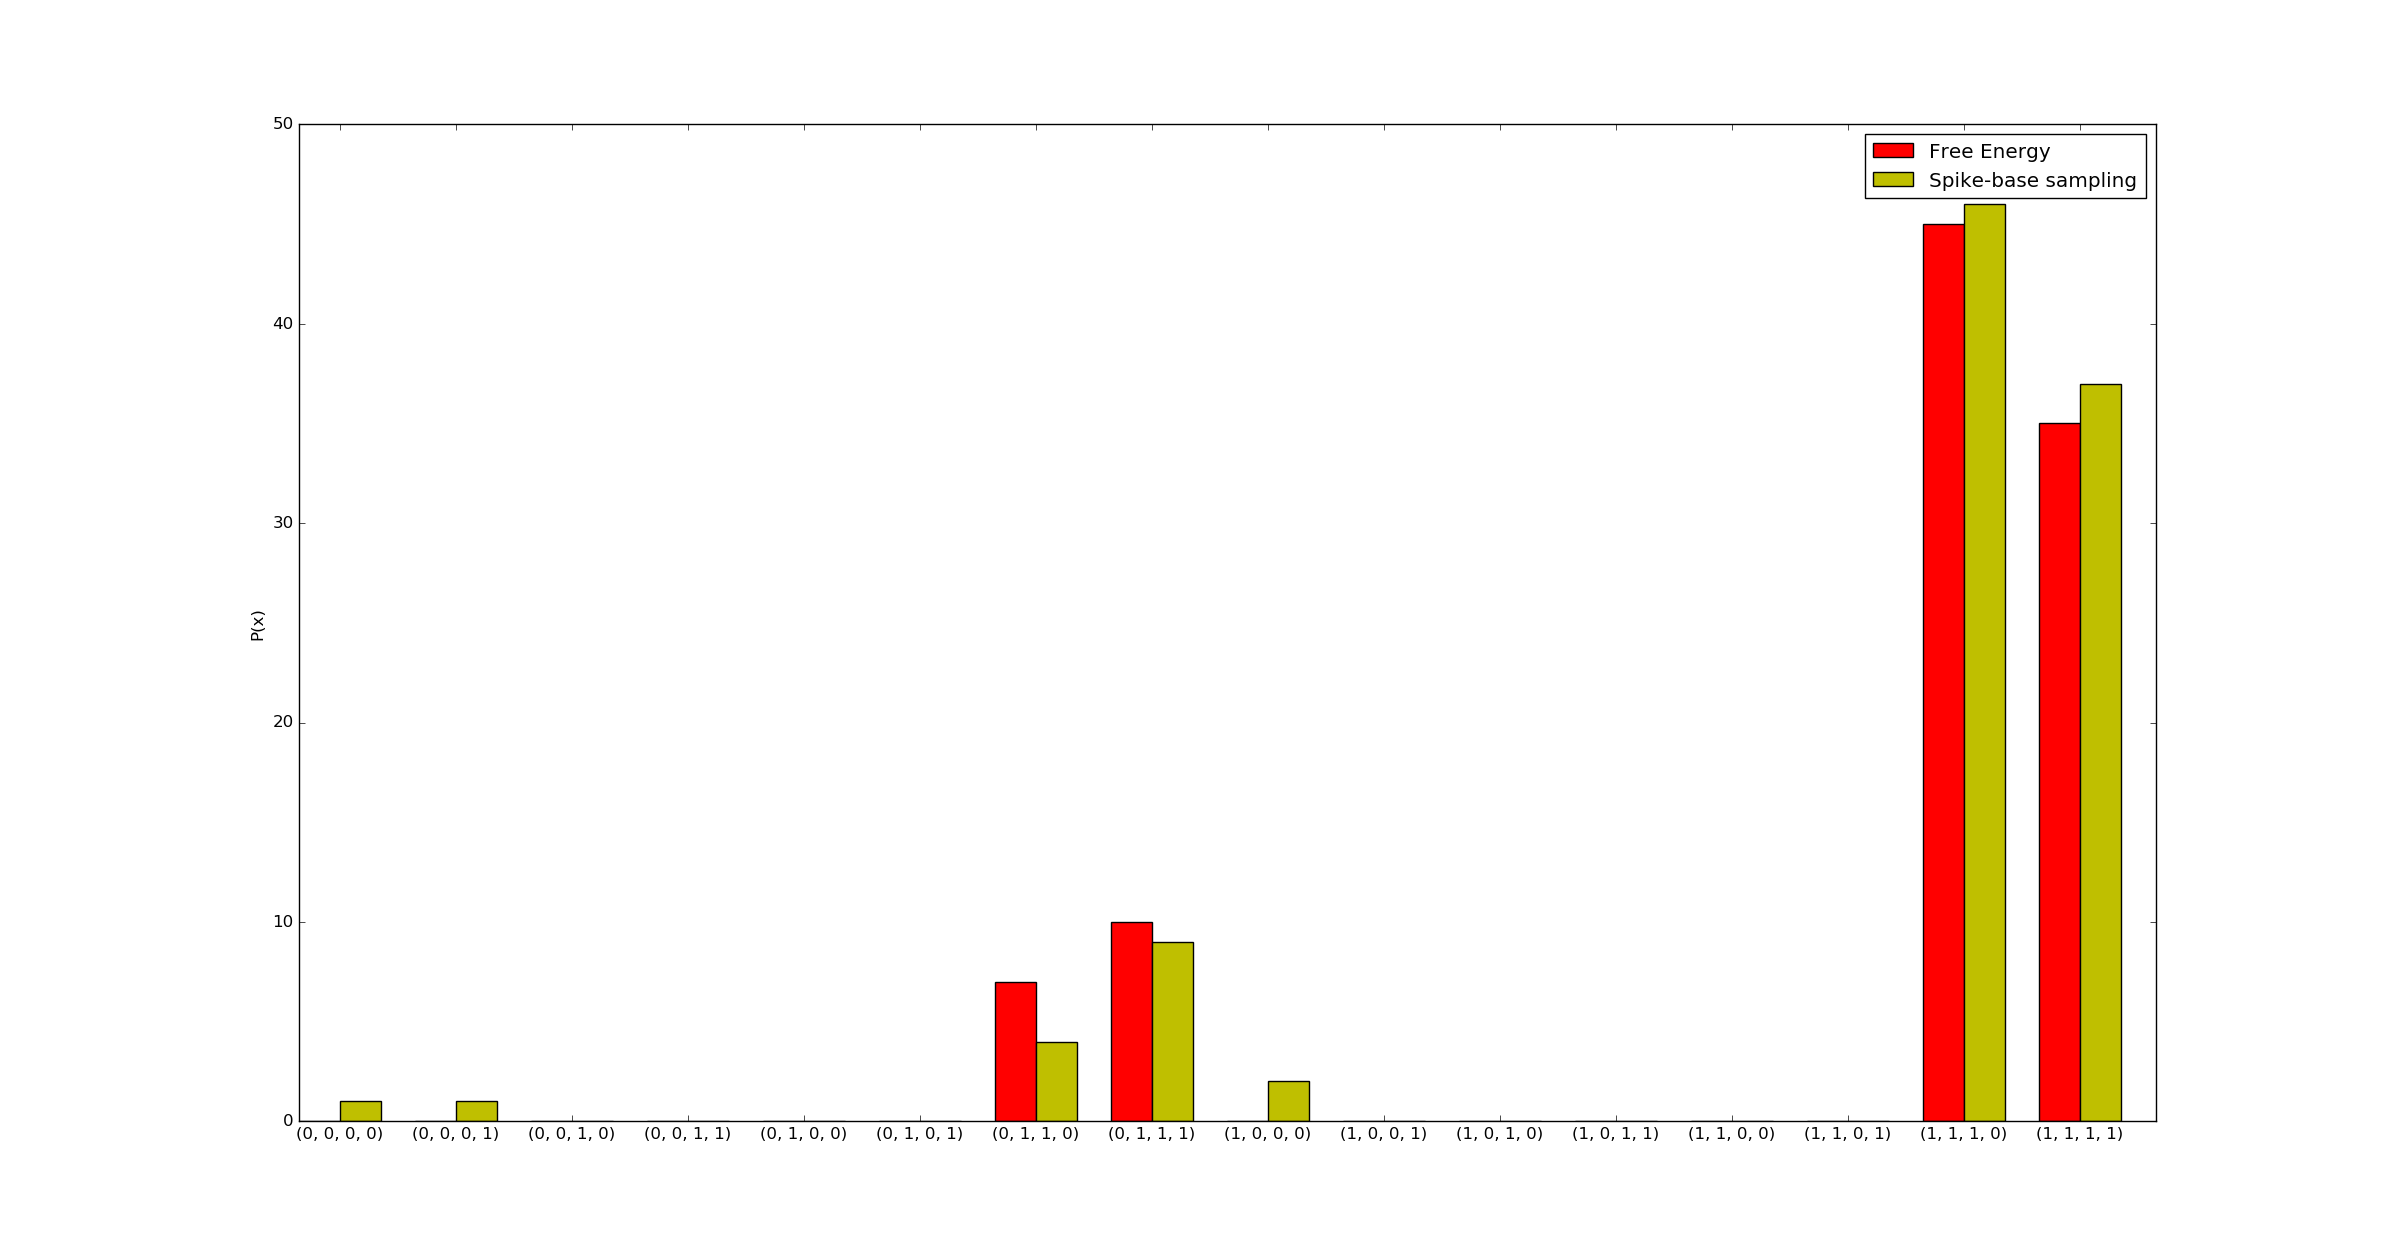
\includegraphics[width=.8\linewidth]{imgs/cuba_lif_bm.png}
  		\caption{Comparison between a HCS CUBA LIF neuron sampling and the true distribution in a RBM.}
  		\label{fig:sub2}
	\end{subfigure}
	\caption{Properties of a current based LIF neuron, put into a simulated high conductance state by high frequency input noise and a artificial high membrane conductance. The neuron also fires with a probability of $0.5$ given no additional input (a) and with input the input output transfer function approximates a sigmoid function (b). A network with such neurons can also to sample in a Boltzmann distribution similar to original distribution (c).}
	\label{fig:cubahcs}
\end{figure}
The DBN conversion is similar to the COBA case, where the COBA neurons are now replaced by the adapted CUBA LIFs (see Fig. \ref{fig:converted2}).

\section{eCD} \label{c:ecdappr}

Another approach implements the learning of the convolutional spiking DBN with an STDP based learning rule. 

The main idea of the learning rule is adapted from Neftcis eCD and applied to a network of LIF neurons with symmetric bidirectional synapses \cite{Neftci2013}.
We modify the STDP learning rule described in Chapter \ref{c:ecd} is used, by extending the model with a learning rate. 
This rule can be reformulated as an iterative rule as follows:
\begin{itemize}
\item The visible unit $v$ spikes: 
\[
\begin{split}
A_v = A_v \exp(\frac{\Delta t}{\tau}) + a_{\delta} ,\\
A_h = A_h \exp(\frac{\Delta t}{\tau}) ,\\
\delta w = g(t) \mu A_v  ,\\
\end{split}
\]
\item The visible unit $h$ spikes: 
\[
\begin{split}
A_h = A_h \exp(\frac{\Delta t}{\tau}) + a_{\delta} ,\\
A_v = A_v \exp(\frac{\Delta t}{\tau}) ,\\
\delta w = g(t) \mu A_h  ,\\
\end{split}
\]
\end{itemize}
where $g(t)$ is the STDP status flag, $\Delta t$ is the time difference to the last previous spike, and $a_{delta}$ represents the input of the incoming spike.


The original division into four training phases poses similarities to pCD since the activity of the hidden layer of the previous step is used as starting state for the next step, we extent the model by a 5th phase between the two data samples, where the model is "flushed" thus enabling normal CD  (see Fig. \ref{fig:ecd5}):

\begin{enumerate}
\item The data signal is applied and the system is allowed to model the data distribution ($g(t)=0$)
\item Positive STDP is used to get $v_i h_j$-data and is added to the weights (postive phase $g(t)=1$)
\item The data signal is remove and the system is allowed to model the model distribution ($g(t)=0$)
\item Negative STDP is used to get $v_i h_j$-model and is subtracted from the synaptic weights (negative phase $g(t)=-1$).
\item The neural activity is "flushed" by inserting a strong negative current into the visible and hidden layer, to learning is performed ($g(t)=0$).
\end{enumerate}

\begin{figure}
	\centering
    	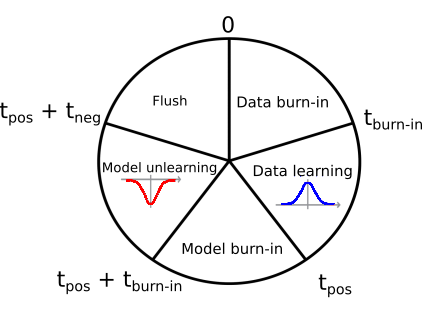
\includegraphics[width=0.4\textwidth]{imgs/eCD_5phases.png} 
    \caption{The five phases for a data sample in the adapted eCD algorithm. }
	\label{fig:ecd5}
\end{figure}

 
\subsection{Convolution in eCD} \label{c:ecdconv}

We implement convolution with local receptive fields and shared weights between synapses through weight synchronization.
Since each weight has their local STDP based update rule (eCD), we have to find a way to synchronize weights between synapses of the same feature map.
To keep the shared weights the same, we perform a weight synchronization step at discrete time steps, since updating all weights after a single update did not show any promising results, due to some self-reinforcement and resulting weight "explosion" (see Fig. \ref{fig:ecdnest} for further insight).
Thus the synchronization at a time step for weight shared weights $w_i$ , $w_j$ can be described by the following rule:  
\[
\begin{split}
w_i(t) = w_{shared}(t-1) + \delta w_i, \\ 
w_j(t) = w_{shared}(t-1) + \delta w_j 
\end{split}
\]
which gives the new shared weight
\[
\begin{split}
w_{shared}(t) = \frac{1}{2} (w_i(t) + w_j(t) ) = \frac{1}{2} (w_{shared}(t-1) + \delta w_i + w_{shared}(t-1) + \delta w_j) = \\ w_{shared}(t-1) + \frac{1}{2} (\delta w_i + \delta w_j).
\end{split}
\]

This results in a update rule similar to the convolutional RBM update rule as in Chapter \ref{c:convrbm}.
Thus we can simply take the mean of the weight changes and apply it to all the weights, which is equivalent to just taking the average of the new individual weights. 

\paragraph{Lateral inhibition} \label{c:latinhib}
In addition we introduce fixed negative connections between neuron in the top/ hidden layers ( which is more biological plausible \cite{King2013} , see a simplified sample in Fig. \ref{fig:bminhib}).
This removes one advantage of RBMs since the hidden layers are no longer independent, which makes it harder to sample from the true distributions, but since the network continuously performs sampling steps, the approximation has shown to be sufficient, if the weights are not too strong and prevent changes of different modes (see Chapter \ref{c:latinhibexp} and Fig. \ref{fig:dbnmixing} ).

\begin{figure}
	\centering
    	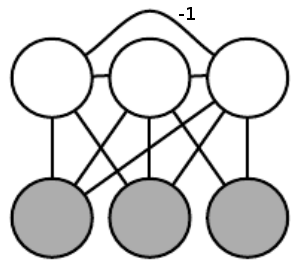
\includegraphics[width=0.4\textwidth]{imgs/lateral_inhib.png} 
    \caption{A (restricted) Boltzmann machine with lateral inhibition in the top layer.}
	\label{fig:bminhib}
\end{figure}


Connecting neurons to neurons on a similar positions in other feature maps appears to make the features more discriminative and less correlated.
Also this poses some similarities to adding a negative structured bias to the hidden units, which has shown to result in better features \cite{NorouziM2009}\cite{LeCun}.

An intuitive interpretation, is that if one feature reacts to a certain input it will be highly active and prevent the others from being active as well and thus prevent them from learning the same features.  

\subsection{Spiking DBNs} \label{c:spikingdbn}

To build up a spiking DBN we train the convolutional BMs layer-wise and forward the input of the previous layer to the next layer.

Either replacing the symmetric bidirectional synapses with forward only synapses or keeping them bidirected, did not show any significant differences (see Fig. \ref{fig:spikingdbnarch} ). 
To be exact the spiking DBN with still bidirectional synapses in the bottom RBMs is a mixture between a deep belief network and a deep Boltzmann machine, since the single Boltzmann machines are still bidirectional connected and only the hidden layer activations are forwarded in a directed manner to the next Boltzmann machines (see Fig. \ref{fig:spikedbn}).

Due to some top-down influences, when stacking a new BM  on the trained BM directly, the hidden distribution gets distorted and unfit input for the new BM to be trained on. 
To solve this in our case we simply use forward connections from the hidden activations to the input layer of a new two layered BM. 
An approach to predict the influences of the top RBM in advance e.g like Salakhutdinovs DBMs with doubling the weights or joint training may sound promising and could be an area for further research \cite{salakhutdinov2009deep}.

\begin{figure}
	\centering
    	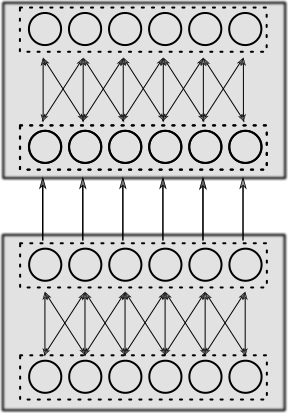
\includegraphics[width=0.4\textwidth]{imgs/spike_dbm.png} 
    \caption{The structure of a deep belief network trained with eCD. The spiking DBN consists of single Boltzmann machines stacked on top of each others. In contrast to artificial DBNs, the Boltzmann machines are still bidirection connected, and two Boltzmann machines are stacked up by forwarding the activations of the hidden layer in the bottom RBM to the visible layer in the top RBM.}
	\label{fig:spikedbn}
\end{figure}

